\subsection{Multi-cluster \& HFL} \label{subsection:eval_multicluster_hfl}

\subsubsection{Classic FL on the Multi-Cluster Setup}

Before analyzing how real HFL performs on multiple clusters, we need to verify that the second setup is capable of classic FL and compare it to the monolith setup.
Observing the aggregated sum of metrics from all three devices leads to flat and less insightful plots.
For this reason, the following graphs will depict the metrics by device.
Figure \ref{fig:eval_7_cpu} shows the CPU utilization of the cluster setup during experiment (7).
It depicts how the control plane root device only manages components but does not perform any heavy operations as intended.
Its CPU utilization is constantly at a very low level.
The orchestrator selected and deployed the image builder service on cluster B.
That is why it is the only busy device during the initial image build phase.
Notably, this scheduling decision seems to be deterministic.
The orchestrator independently selected Cluster B for every single run.
Once FL actor deployment and training start, CPU utilization gets distributed among both cluster nodes.
Figure \ref{fig:eval_7_mem} shows the memory utilization of the devices.
The memory stays stable when no workloads are performed on a device, which is the case for the root at all times and for cluster-A while cluster-B is building the images. 
The reason why the root device has a higher memory usage then the two clusters is because the root hosts the control plane.
This includes Oakestra's root orchestrator and all FLOps management components.

Figure \ref{fig:eval_7_disk_space} shows the increase in disk space for the devices.
It shows how cluster-B's disk space is increasing during the build process due to the dependencies and layers that are pulled and build.
There is a drop after the build process finishes, and the builder service is undeployed.
In the middle of the build process, cluster B pushes the built base image to the root that hosts the image registry.
Cluster-B pushes the FL-actor images without a significant increase because the common base layers are reused.
The disk space of cluster-A only starts increasing when the FL actors are deployed on it.
Figures \ref{fig:eval_7_net_received} and \ref{fig:eval_7_net_send} show the received and sent network changes on the devices, matching the disk space changes.
The FLOps stages seen in Figure \ref{fig:eval_7_stage_durations} of experiment (7) do not show any remarkable outliers and resemble the base case.
The only difference is that the project and its stages take longer due to the weaker hardware.
Project stages on our multi-cluster setup take approximately 0.67 to 7.5 (average 2.88) times longer than on the monolith setup.
Because stages have different durations and weights the overall runtime of a project only increased by approximately 1.67 times.
The final training results are equivalent to (1).



\begin{figure}[p]

    \begin{adjustwidth}{-0.2\paperwidth}{-0.2\paperwidth}
        \centering
        % 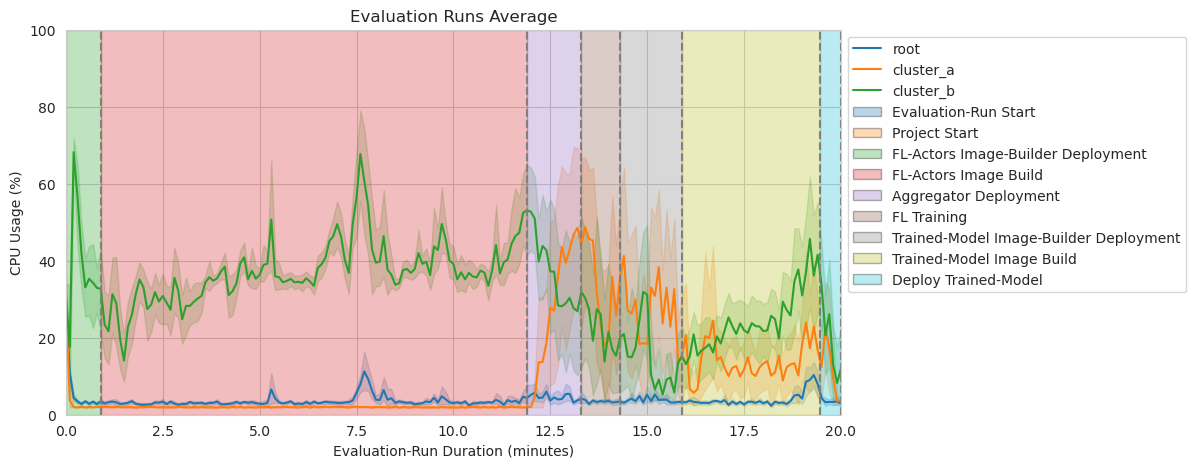
\includegraphics[width=0.95\paperwidth]{evaluations/multicluster_hfl/eval_9_7_simple_multicluster_cpu_split.png}
        \includegraphics[width=0.85\paperwidth]{evaluations/experiment_7/cpu.pdf}
        \caption{Experiment 7: CPU Utilization}
        \label{fig:eval_7_cpu}
    \end{adjustwidth}

    \begin{adjustwidth}{-0.2\paperwidth}{-0.2\paperwidth}
        \centering
        \includegraphics[width=0.85\paperwidth]{evaluations/experiment_7/mem.pdf}
        \caption{Experiment 7: Memory Utilization}
        \label{fig:eval_7_mem}
    \end{adjustwidth}

    \begin{adjustwidth}{-0.2\paperwidth}{-0.2\paperwidth}
        \centering
        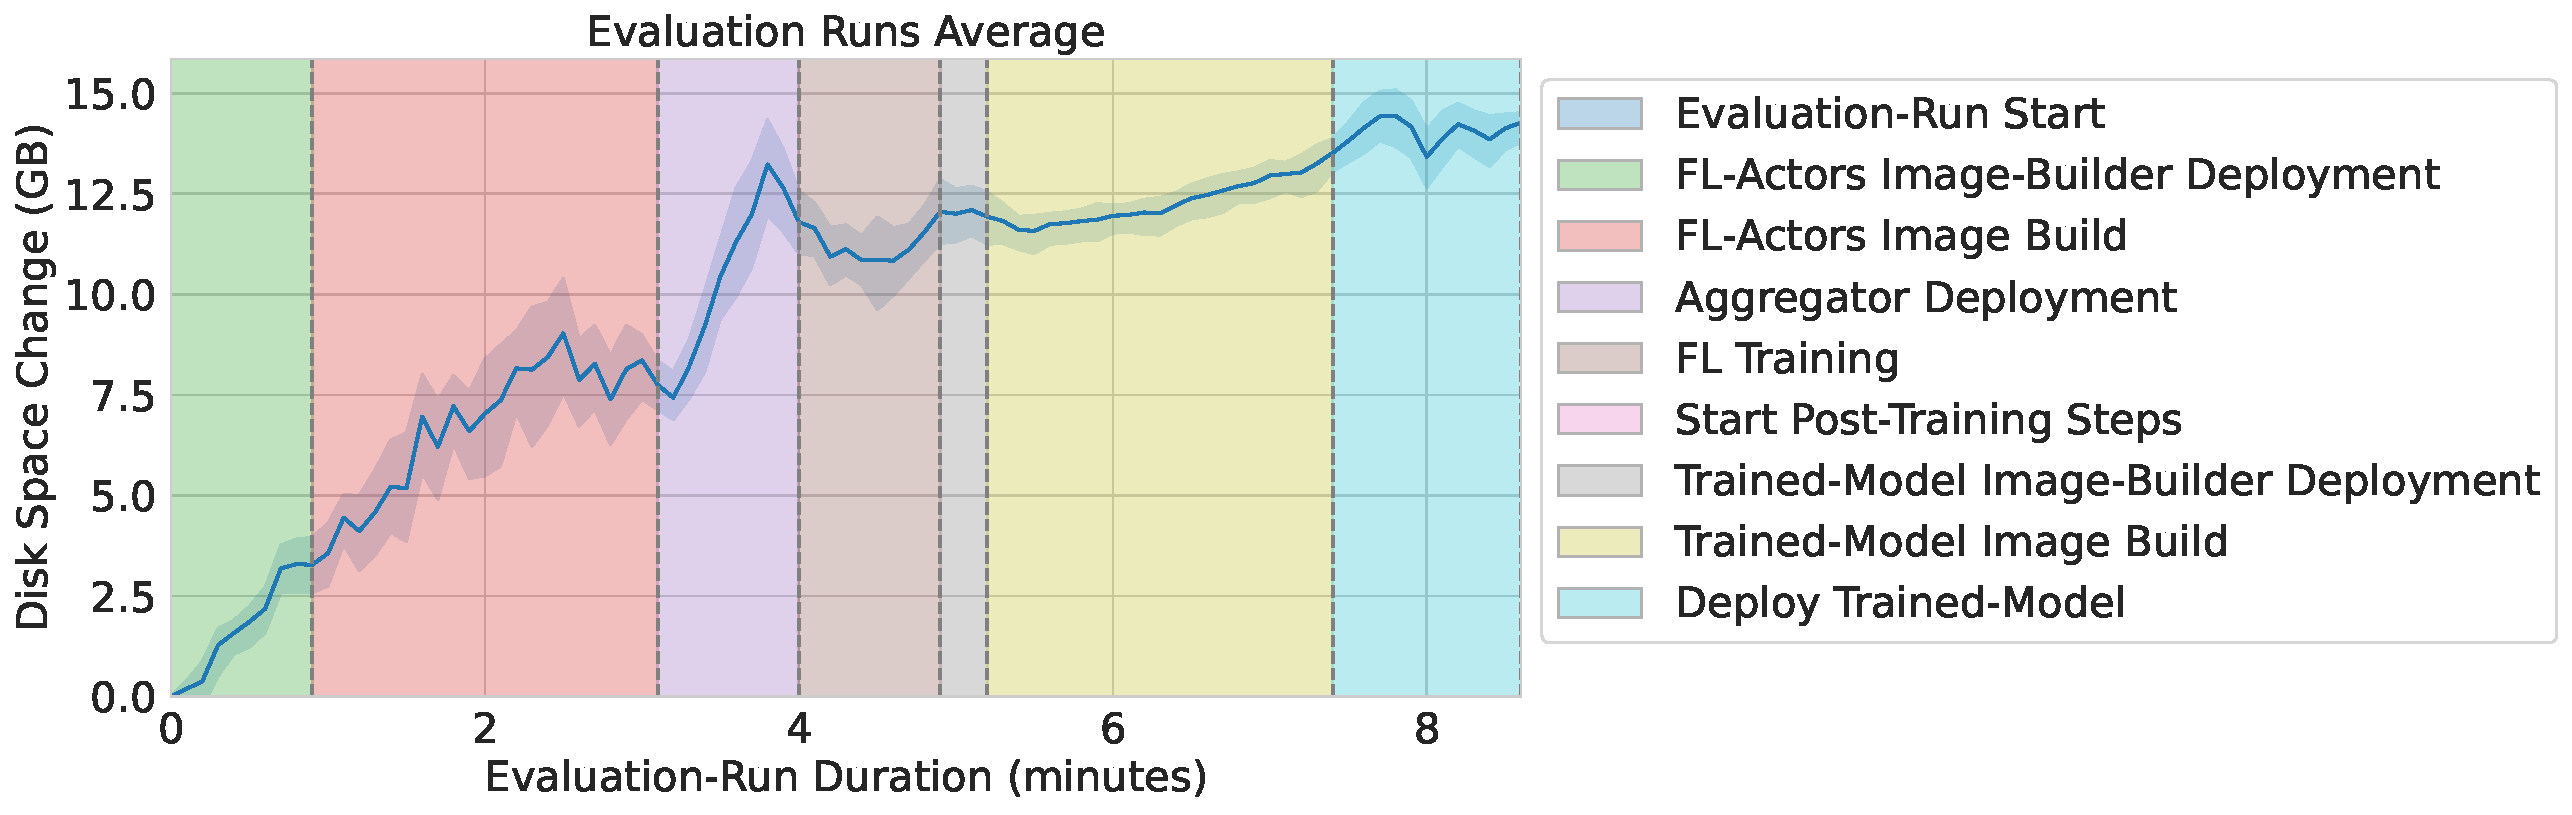
\includegraphics[width=0.85\paperwidth]{evaluations/experiment_7/disk.pdf}
        \caption{Experiment 7: Disk Space}
        \label{fig:eval_7_disk_space}
    \end{adjustwidth}
\end{figure}

\begin{figure}[p]
    \begin{adjustwidth}{-0.2\paperwidth}{-0.2\paperwidth}
        \centering
        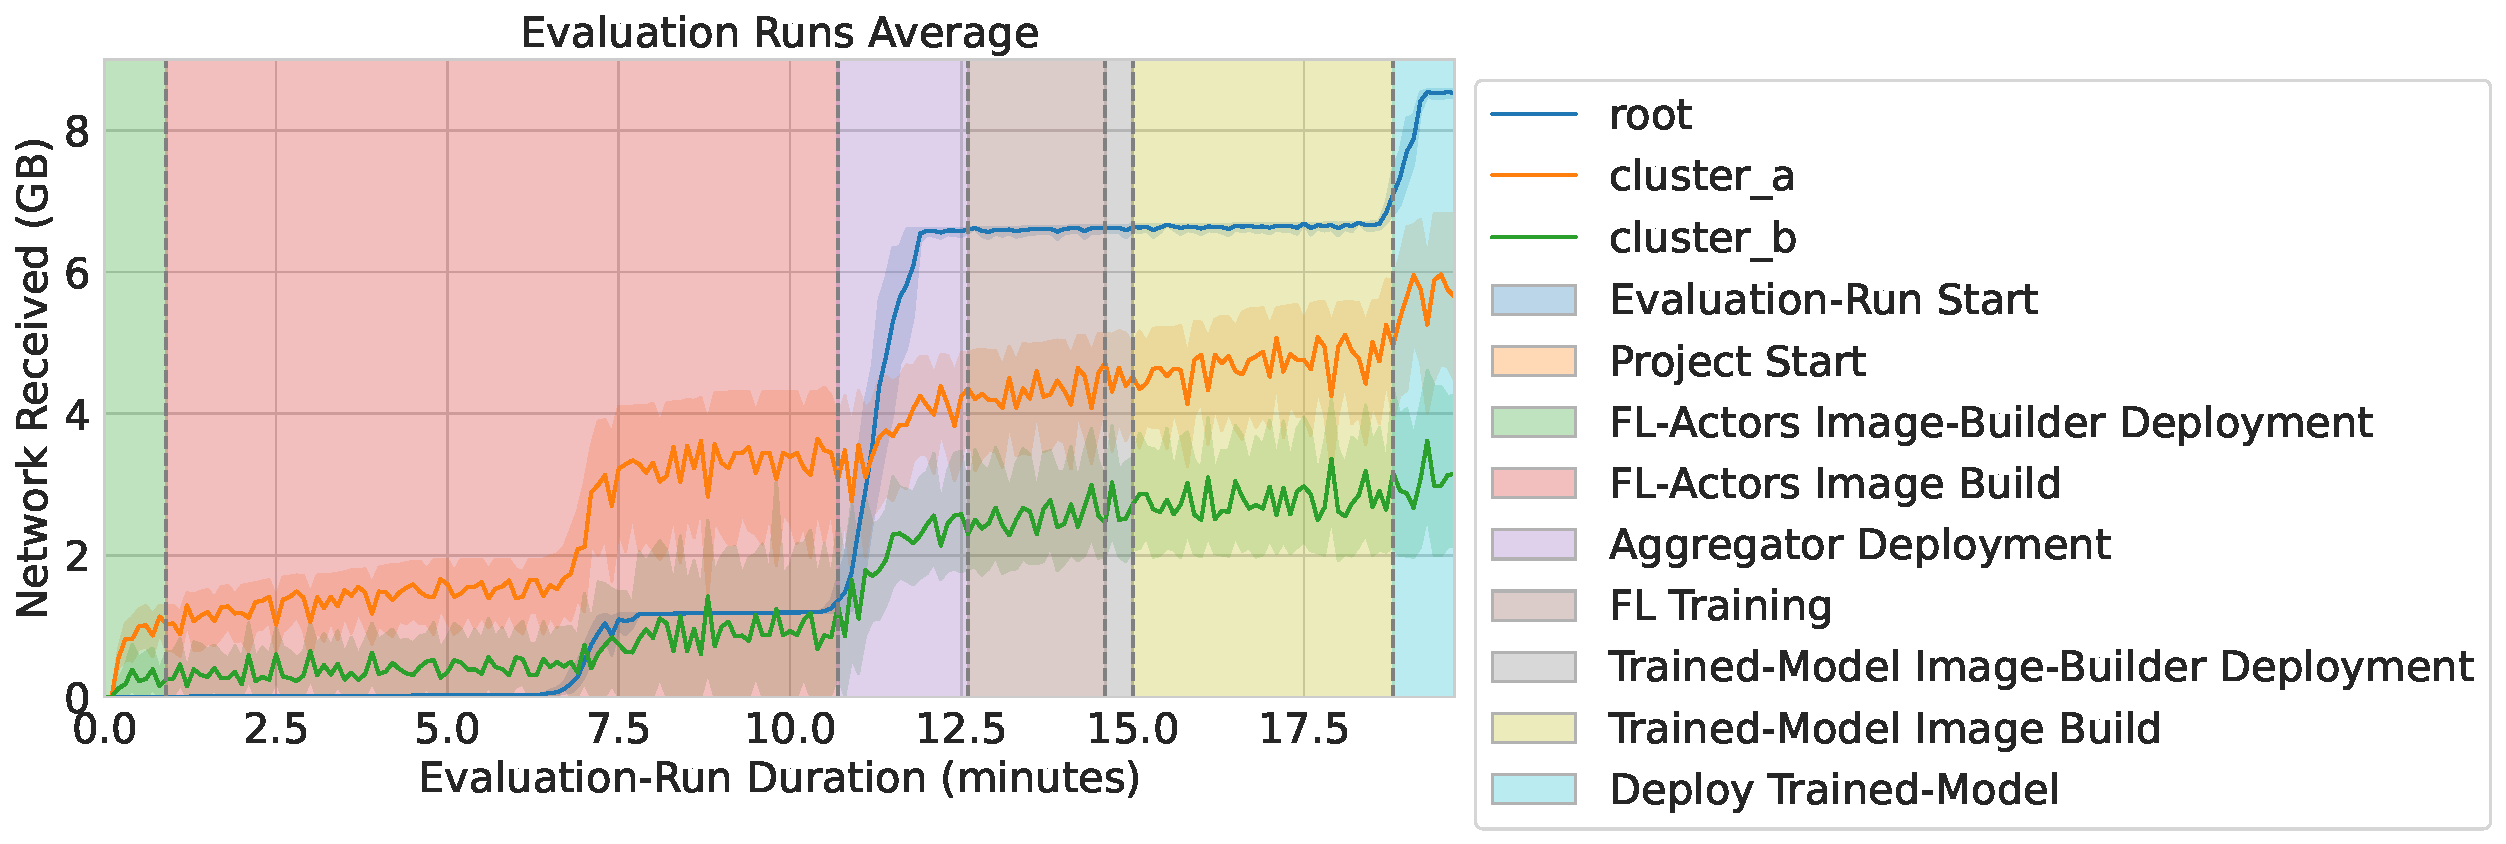
\includegraphics[width=0.83\paperwidth]{evaluations/experiment_7/net_received.pdf}
        \caption{Experiment 7: Received Network}
        \label{fig:eval_7_net_received}
    \end{adjustwidth}

    \begin{adjustwidth}{-0.2\paperwidth}{-0.2\paperwidth}
        \centering
        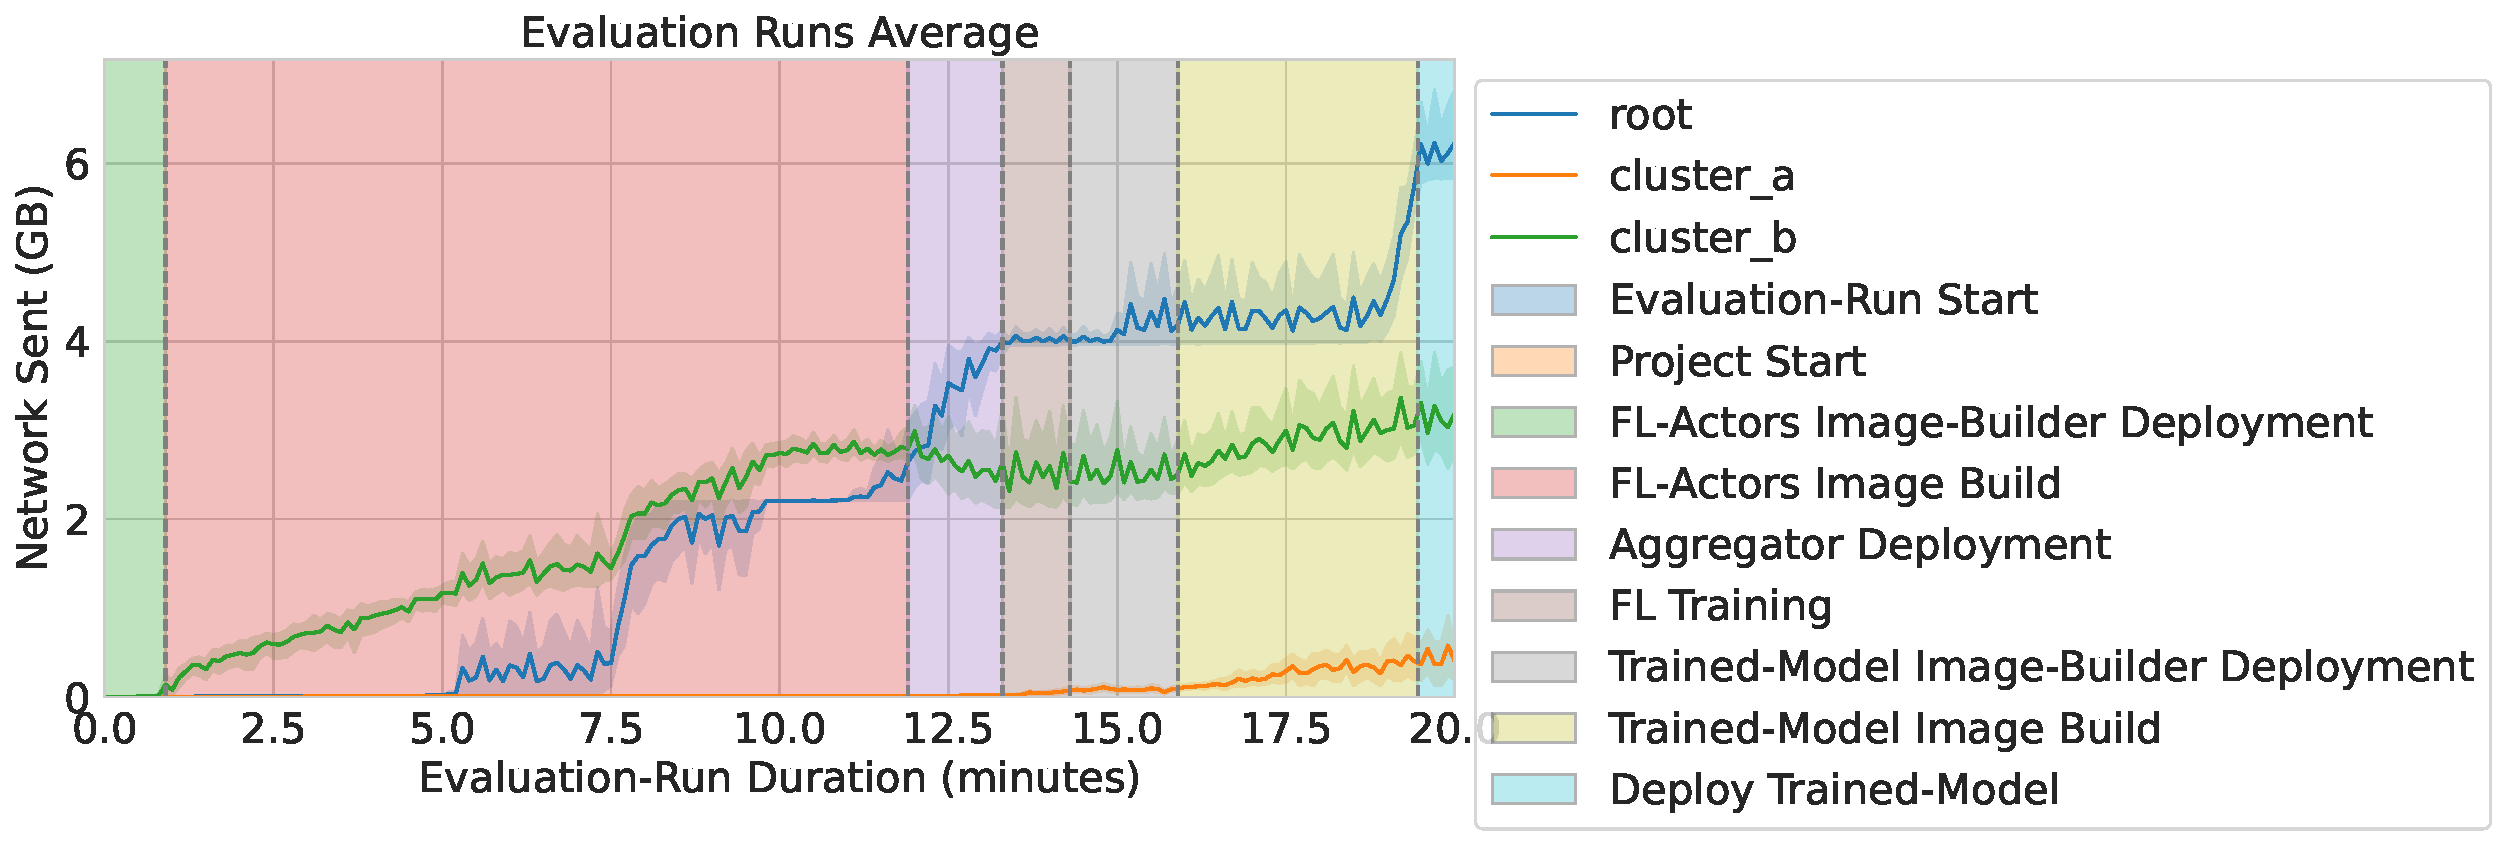
\includegraphics[width=0.83\paperwidth]{evaluations/experiment_7/net_sent.pdf}
        \caption{Experiment 7: Send Network}
        \label{fig:eval_7_net_send}
    \end{adjustwidth}

    \begin{adjustwidth}{-0.2\paperwidth}{-0.2\paperwidth}
        \centering
        \includegraphics[width=0.80\paperwidth]{evaluations/experiment_7/stage_durations.pdf}
        \caption{Experiment 7: Stage Durations}
        \label{fig:eval_7_stage_durations}
    \end{adjustwidth}
\end{figure}

\pagebreak

\subsubsection{Minimal HFL base-case on a monolith Cluster}

\begin{figure}[H]
    \begin{adjustwidth}{-0.2\paperwidth}{-0.2\paperwidth}
        \centering
        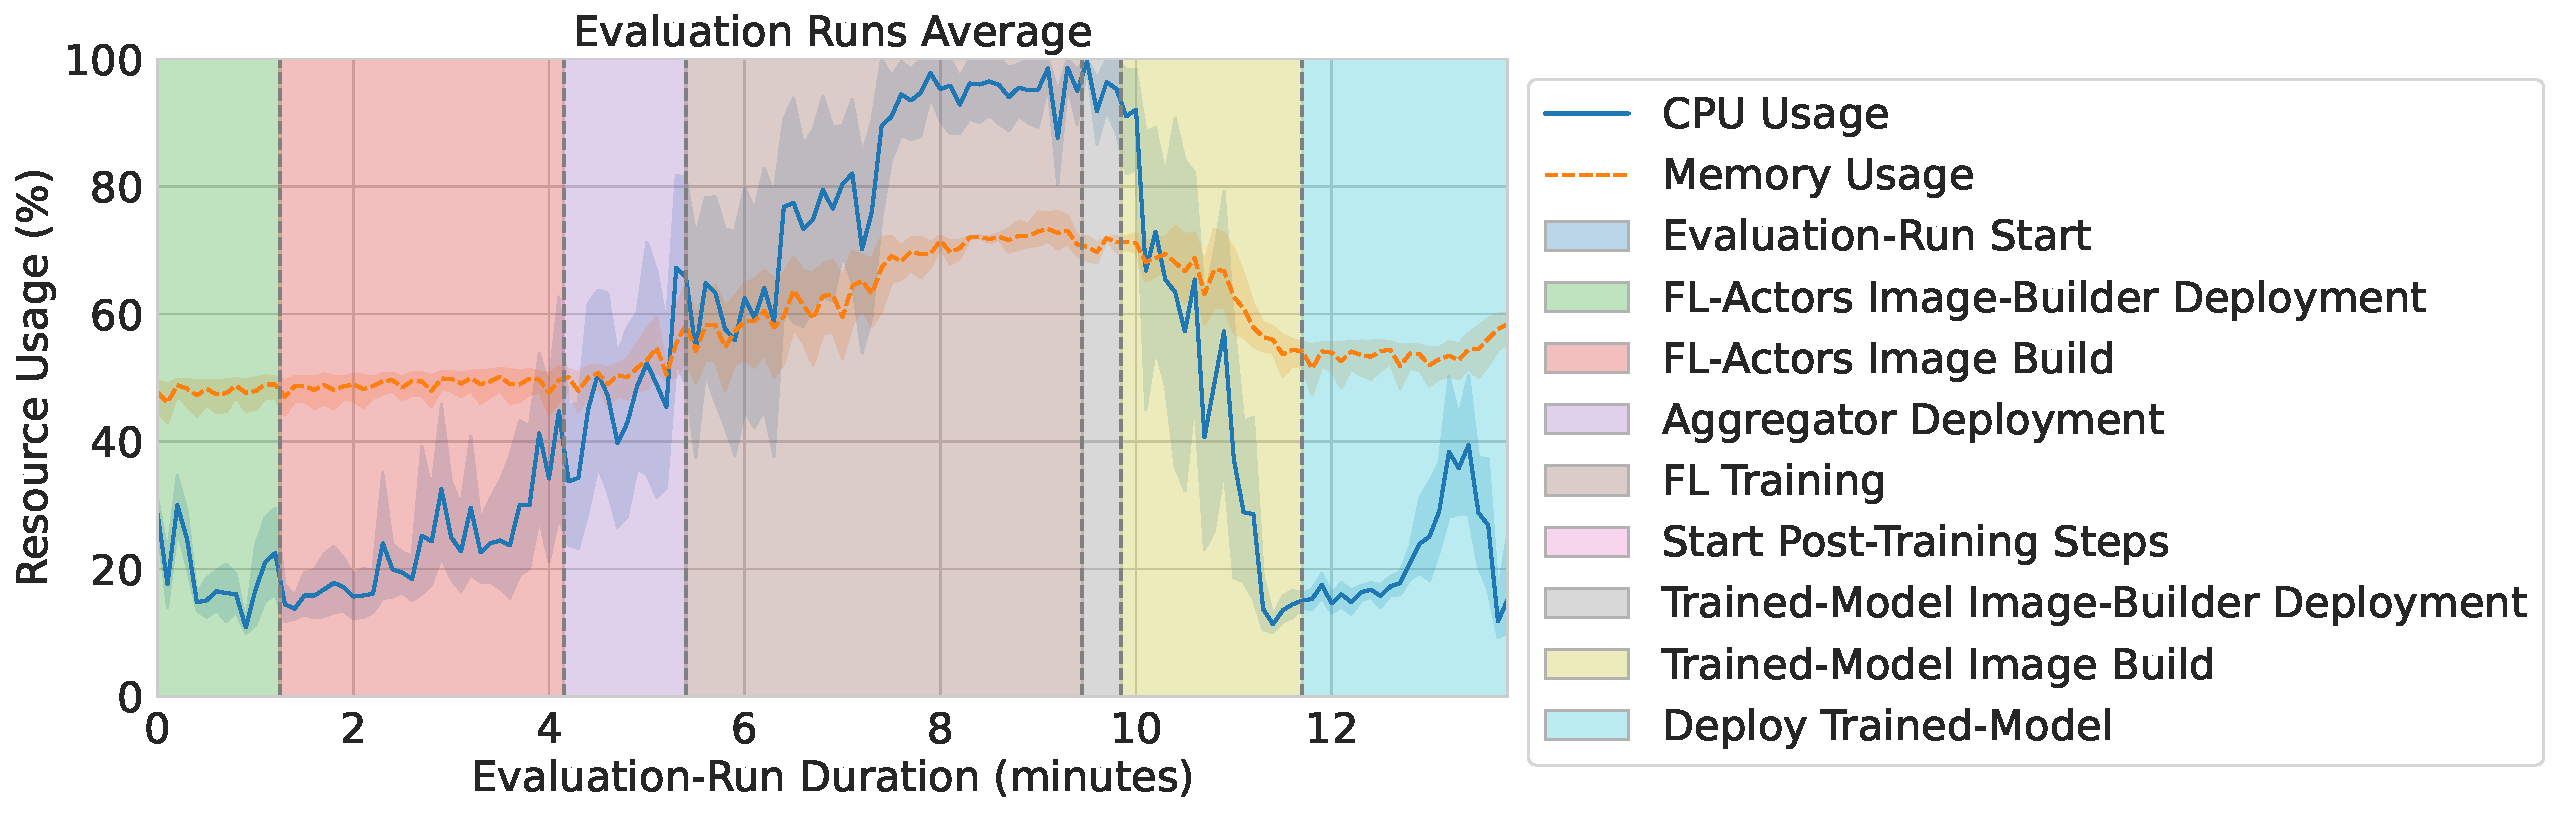
\includegraphics[width=0.95\paperwidth]{evaluations/experiment_6/cpu_mem.pdf}
        \caption{Experiment 6: Monolith HFL CPU \& Memory}
        \label{fig:eval_6_cpu_mem}
    \end{adjustwidth}
\end{figure}

Figure \ref{fig:eval_6_cpu_mem} shows the CPU and memory utilization of experiment (6).
Its purpose is to be a minimal HFL base-case that only uses a single cluster.
In additon, this experiment proofs that FLOps' custom clustered HFL solution works.
Compared to (1) the project duration is a bit longer due to the longer training stage.
Every other metric stays similar to (1).
This includes the stage durations, disk space, net IO, and training results.
CPU and memory utilization are slightly increased in the deployment and training stages because of more FL actors.


\subsubsection{HFL on the Multi-Clustered Setup}

Figure \ref{fig:eval_8_cpu} shows the CPU utilization of the multi-cluster setup devices during HFL.
The image build seems to be no longer handled by a single cluster but is more distributed among both.
In (7), learners were randomly deployed on clustered.
In (8), the figure clearly shows that the CPU is utilized more and distributed more equally among the clusters.
This is the case because each cluster gets its own cluster aggregator and set of learners.
This more homogeneous utilization also applies to memory, as Figure \ref{fig:eval_8_mem} shows.
All other metrics show a similar change from (7) to (8) as from (1) to (6).
This includes disk space, net IO, stage durations (Figure \ref{fig:eval_8_stage_durations}), and training results.
These findings prove that FLOps can perform clustered HFL on distributed multi-cluster devices.


\begin{figure}[p]
    \begin{adjustwidth}{-0.2\paperwidth}{-0.2\paperwidth}
        \centering
        \includegraphics[width=0.85\paperwidth]{evaluations/experiment_8/cpu.pdf}
        \caption{Experiment 8: Multi-Cluster HFL CPU Utilization}
        \label{fig:eval_8_cpu}
    \end{adjustwidth}

    \begin{adjustwidth}{-0.2\paperwidth}{-0.2\paperwidth}
        \centering
        \includegraphics[width=0.85\paperwidth]{evaluations/experiment_8/mem.pdf}
        \caption{Experiment 8: Multi-Cluster HFL Memory Utilization}
        \label{fig:eval_8_mem}
    \end{adjustwidth}

    \begin{adjustwidth}{-0.2\paperwidth}{-0.2\paperwidth}
        \centering
        \includegraphics[width=0.80\paperwidth]{evaluations/experiment_8/stage_durations.pdf}
        \caption{Experiment 8: Stage Durations}
        \label{fig:eval_8_stage_durations}
    \end{adjustwidth}
\end{figure}